When two immiscible fluids are mixed, they phase separate into fluid domains to reduce the interfacial energy between them. This phenomena is driven by the free energy
reduction as the interface area between both fluids decrease. To inhibit this process, stabilizers such as small-molecule surfactants, particles, or biopolymers are commonly introduced. 
Surfactants, for example, reduce the surface tension between the dispersed and continuous phases, thereby lowering the interfacial energy and promoting the stability of emulsions. 
A familiar example is soap, which facilitates the emulsification of dirt into droplets suspended in water through mechanical agitation.
Without such additives, the dispersed phase tends to coalesce in order to reduce interfacial area. While surfactants and biopolymers reduce interfacial tension, particle stabilizers 
function by adsorbing at the interface and effectively reducing the interfacial area between fluid domains. The free energy associated with the decrease in interfacial area 
can be orders of magnitude larger than the thermal energy of the system $k_b T$ which makes the particle irreversibly adsorbed on the interface \cite{ngai_particle-stabilized_2015}.

Compared to surfactant-stabilized emulsions, particle-stabilized emulsions (Pickering emulsions) exhibit enhanced resistance to coalescence and coarsening
due to the irreversibility of particle adsorption at the interface \cite{ngai_particle-stabilized_2015} .
Additionally, growing environmental and toxicity concerns surrounding small-molecule surfactants have increased interest in particle-stabilized emulsions, due to their lower toxicity, 
enhanced biocompatibility, and potential for sustainable sourcing from renewable materials such as chitin and cellulose.
\cite{kaczerewska_environmental_2020, lechuga_acute_2016, fujisawa_nanocellulose-stabilized_2017, tang_stimuli-responsive_2016, kalliola_carboxymethyl_2018}.
The microstructure of Pickering emulsions has been extensively studied, notably by Binks and Lumsdon in the early 2000s. Their investigations revealed that the emulsion droplet radius 
follows the relationship $R_e \propto \frac{1}{\phi_p}$, where $\phi_p$ represent the volume fractions of particles \cite{binks_pickering_2001}. 
They also identified key parameters influencing microstructure, such as fluid composition and particle wettability. Neutrally wetting particles tend to stabilize nearly spherical droplets, 
while non-neutrally wetting particles can induce curvature, leading to the formation of bridged droplets, capillary aggregates, and other anisotropic structures, as illustrated in 
Figure~\ref{fig:state_diagram_particle_emulsions}.

\begin{figure}
    \centering
    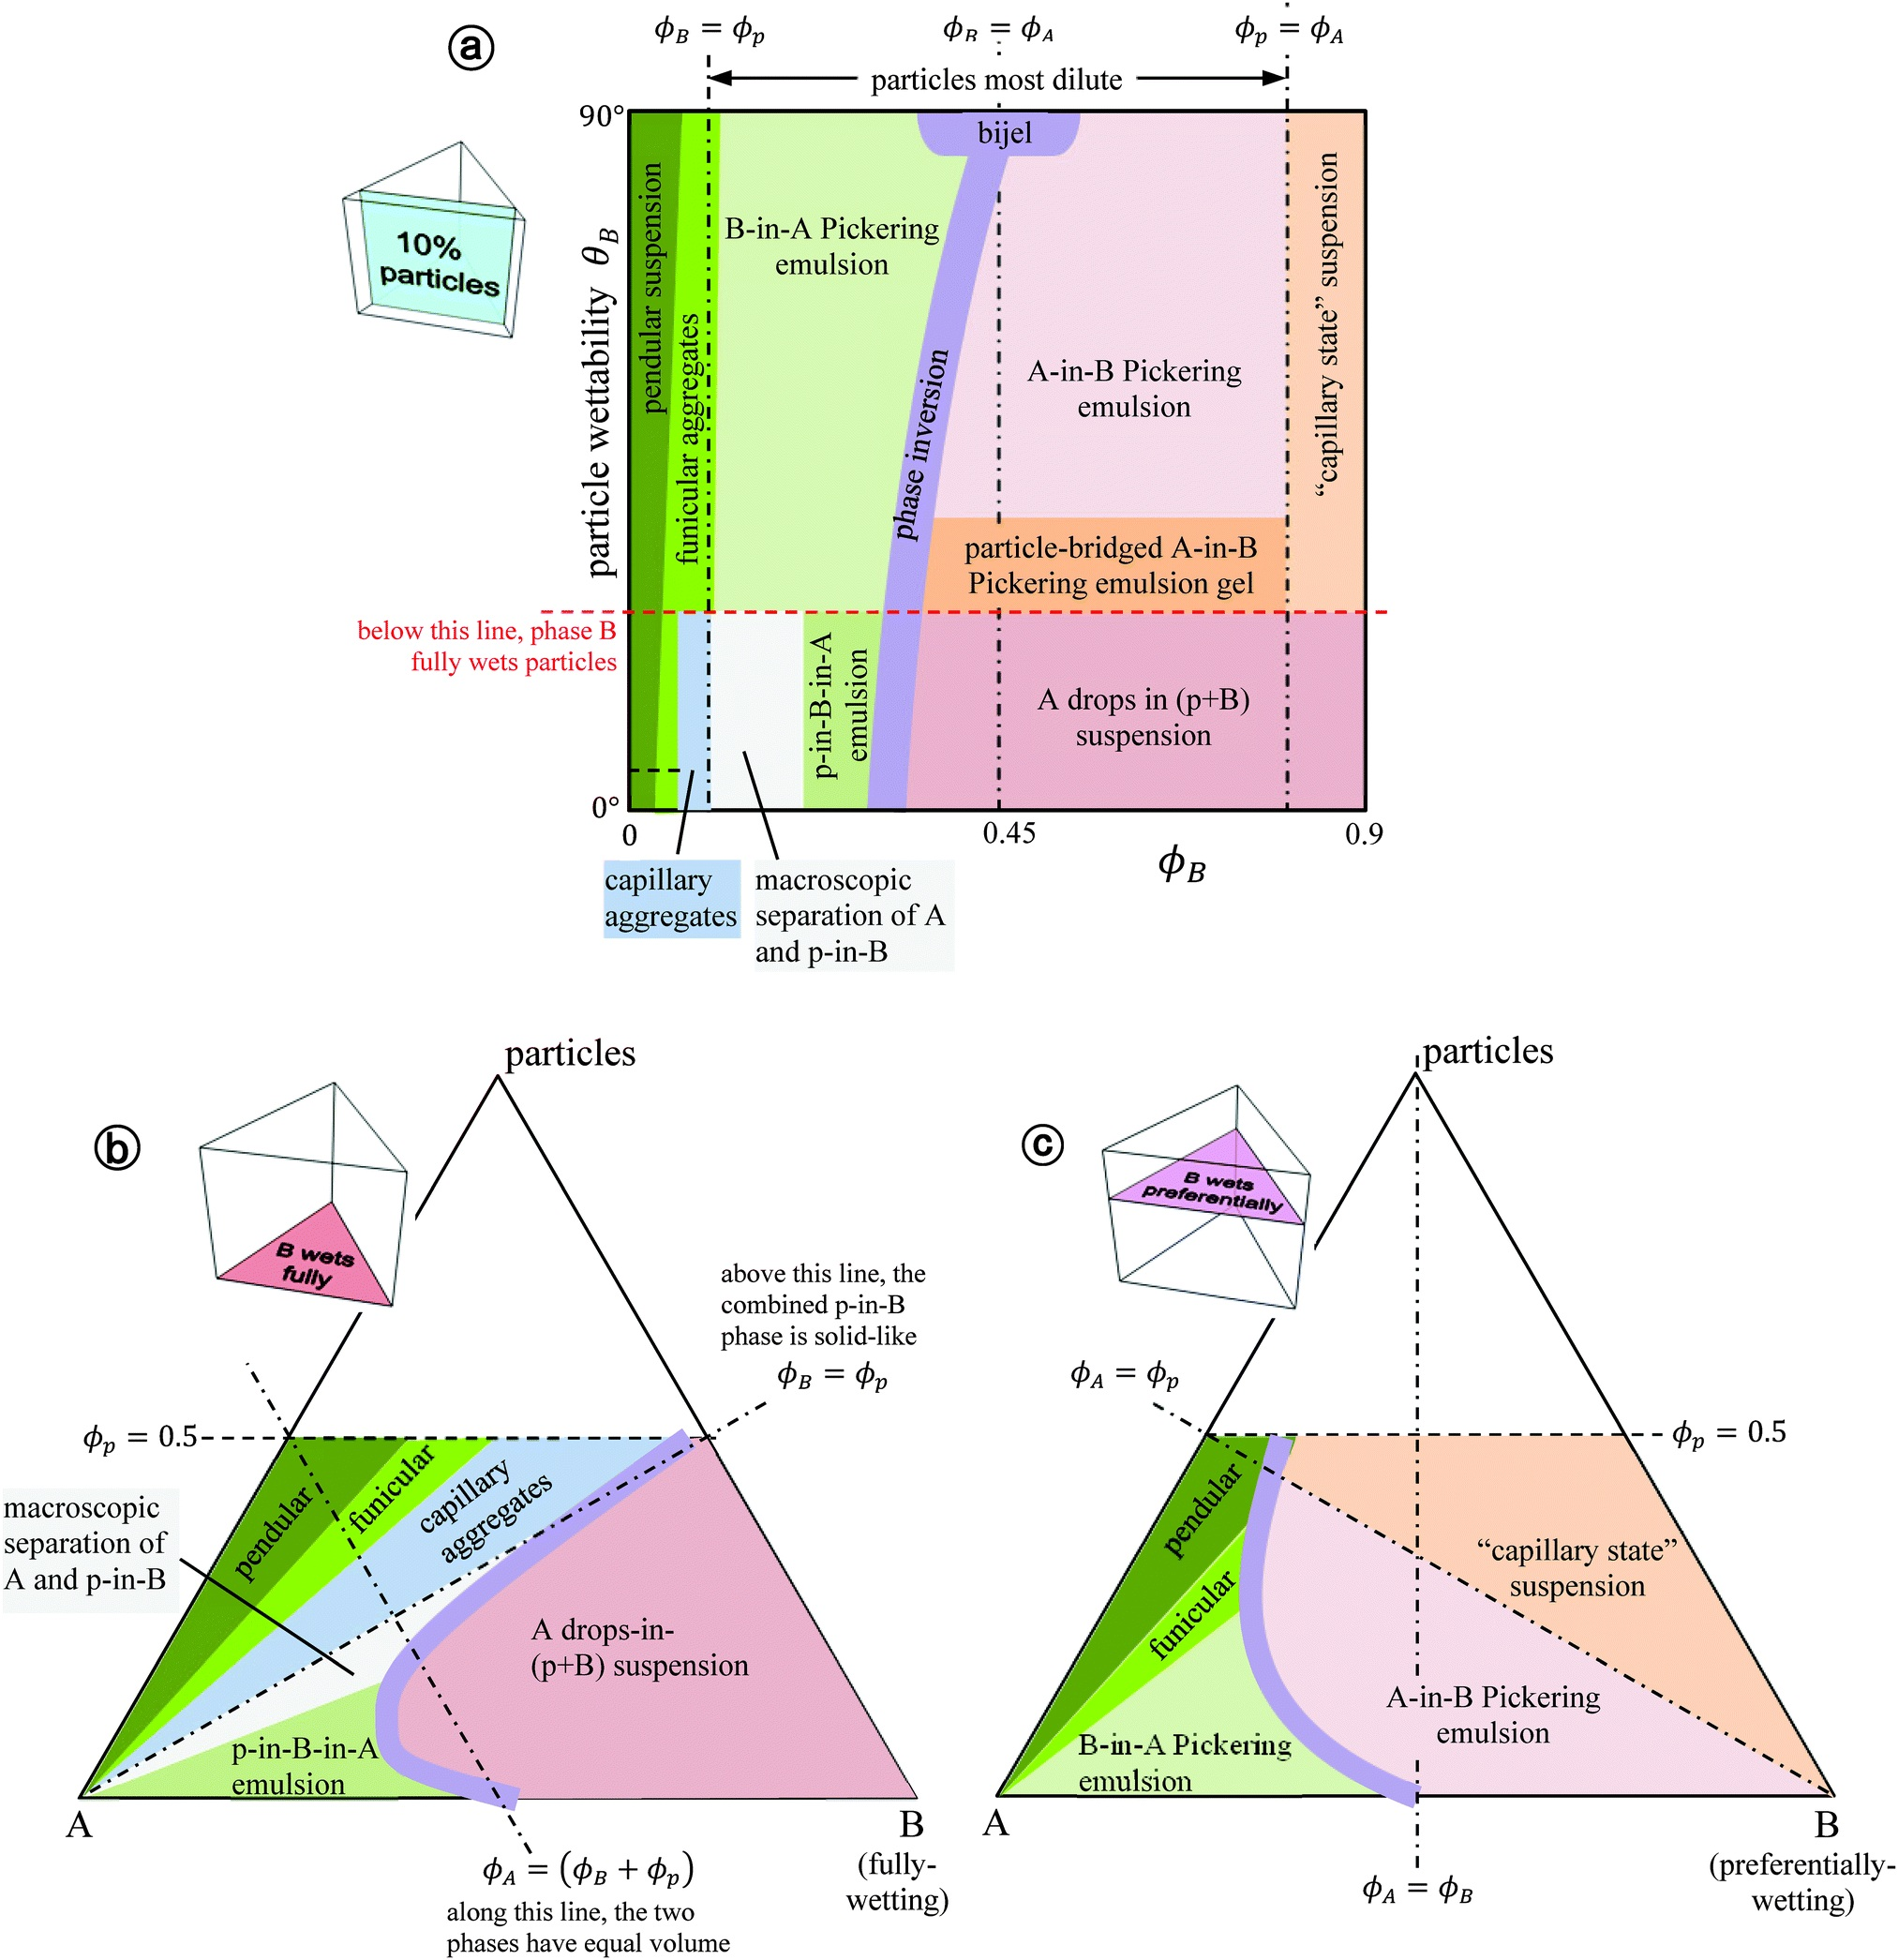
\includegraphics[scale = 0.3]{figures/literature_review/state_diagram.jpg}
    \caption{Formation criteria for a particle stabilized emulsion that can form bijel. Reprinted Figure 3 with permission from the Royal Society of Chemistry from 
             \textit{Velankar, S. S. A Non-Equilibrium State Diagram for Liquid/Fluid/Particle Mixtures. Soft Matter 2015, 11 (43), 8393-8403}
             with permission from the Royal Society of Chemistry under license number 1551968-1; Permission conveyed through Copyright Clearence Center}
    \label{fig:state_diagram_particle_emulsions}
\end{figure}

One microstructure of interest shown in Figure~\ref{fig:state_diagram_particle_emulsions} is the bicontinuous interfacially jammed emulsion gel (bijel). This unique microstructure was 
first identified in 2005 by Stratford et al., who used a multicomponent Lattice Boltzmann method coupled with suspended particles to simulate the 
dynamics of particle-stabilized emulsions under these conditions \cite{stratford_colloidal_2005}. Their simulations revealed that, following the onset of spinodal decomposition, particles 
rapidly adsorb at the evolving fluid-fluid interface. When the available interfacial area becomes comparable to the total cross-sectional area of the particles, coarsening is arrested, 
resulting in a jammed, tortuous, co-continuous morphology characteristic of bijels (see Figure~\ref{fig:bijel_coarsen}).

\begin{figure}
    \centering
    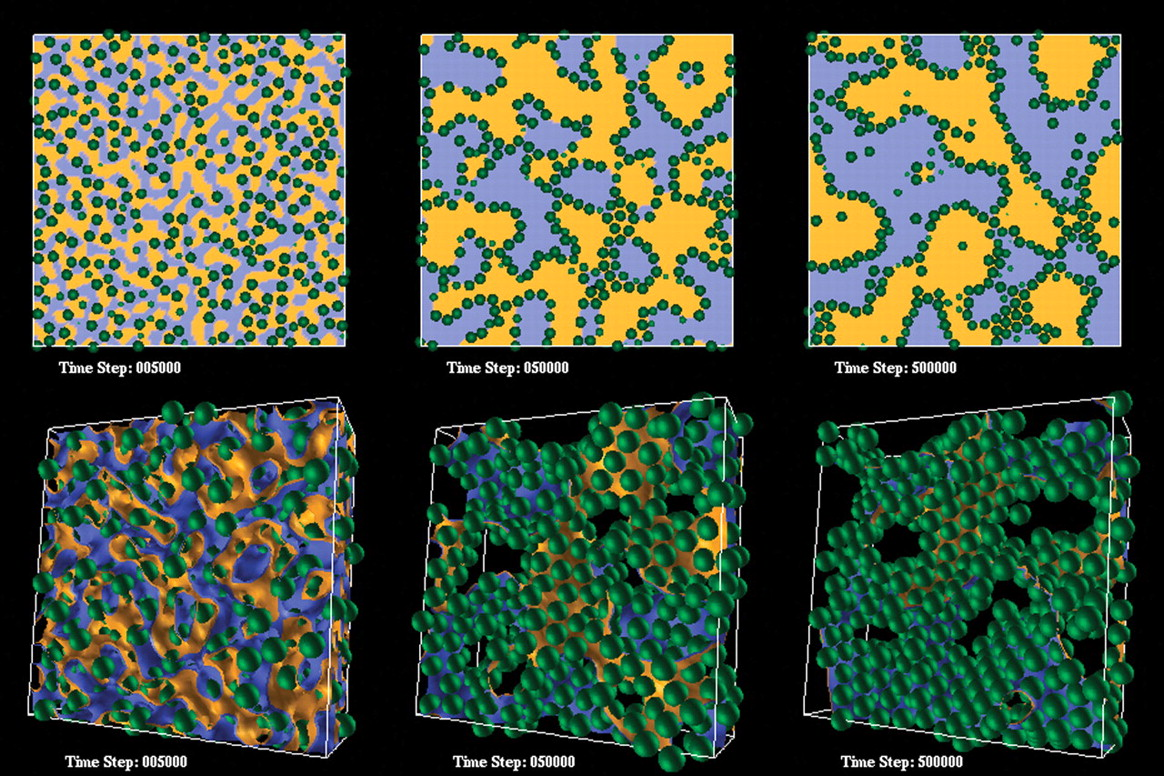
\includegraphics[scale = 0.3]{figures/introduction/bijel_coarsening.jpg}
    \caption{Initiation and arrest of spinodal decomposition as particles adsorb onto the interface, followed by jamming once the 
            interfacial area matches the cross sectional area of the adsorbed particles. Reprint of Figure 1 from
            \textit{Stratford, K.; Adhikari, R.; Pagonabarraga, I.; Desplat, J.-C.; Cates, M. E. Colloidal Jamming at Interfaces: A Route to Fluid-Bicontinuous Gels. Science 2005, 309 (5744), 2198-2201}
            Reprinted with permission from AAAS under license number 5966820525314.}
    \label{fig:bijel_coarsen}
\end{figure}

Bijel microstructures are of interest because their bicontinuous, interpenetrating networks enable tunable transport and separation properties. The computational discovery of the technique to 
synthesize bijels was succeeded by the experimental synthesis of a bijel in 2007 by Herzig et al., who used a 2,6-lutidine/water system stabilized with surface-modified silica particles
\cite{herzig_bicontinuous_2007}.
This binary fluid system exhibits a lower critical solution temperature (LCST) of 34.1\textdegree C and a critical composition at approximately 28\% lutidine by weight. By preparing the mixture at this 
critical composition and heating it past the LCST, phase separation was induced in a process known as Thermally Induced Phase Separation (TIPS). The system underwent coarsening until particle
interactions at the interface jammed the microstructure in place, once the cross-sectional area of the particles matched the interfacial area, forming a bijel. Since this initial 
experimental synthesis, TIPS has been widely used in laboratory-scale studies to synthesize a variety of small molecule, oligomeric, and polymeric systems 
\cite{tavacoli_novel_2011, lee_bicontinuous_2010, bai_dynamics_2015, ching_rapid_2021}. 

However, industrial applications require continuous, scalable fabrication techniques capable of generating application specific tailored microstructures. The thermal induction of phase separation
does not permit easy scale up due to limitations of suitable systems that forms bijels and the need to have constant cooling rates to ensure consistent microstructures through the entire reaction
vessel. Solvent Transfer Induced Phase Separation (STrIPS) has emerged as a promising solution to address these issues.
As illustrated in Figure~\ref{fig:strips}, STrIPS involves a ternary fluid system composed of two immiscible fluids 
and a solvent. In the initial stage (Figure~\ref{fig:strips}a), a casting mixture is prepared. Phase separation is then triggered by flowing a co-solvent past the mixture to extract the solvent 
(Figure~\ref{fig:strips}b). This solvent transfer must occur within the spinodal region of the ternary phase diagram to ensure spinodal decomposition. By adjusting flow rates of both the casting 
mixture and the solvent removal stream, the resulting bijel morphology can be finely controlled. STrIPS has been successfully employed in applications ranging from battery electrode templating to drug 
delivery systems, liquid-in-liquid printing, and the creation of intrinsically polymerizable bijels for freestanding structures 
\cite{garcia_scalable_2019, thorson_bijel-templated_2019, amirfattahi_fabrication_2024, ching_rapid_2021}. The method is flexible with respect to fluid choice, with 
the only requirement being a well-characterized phase diagram that keeps the system within the spinodal regime throughout the solvent exchange process. Other techniques based on
induced phase separation such as Vapor Induced Phase Separation(VIPS) and controlled coalescence of droplets to form bijels through shear (homogenization) have also been identified as techniques
to synthesize bijels \cite{wang_scalable_2020, huang_bicontinuous_2017, cai_bijels_2017}.

\begin{figure}
    \centering
    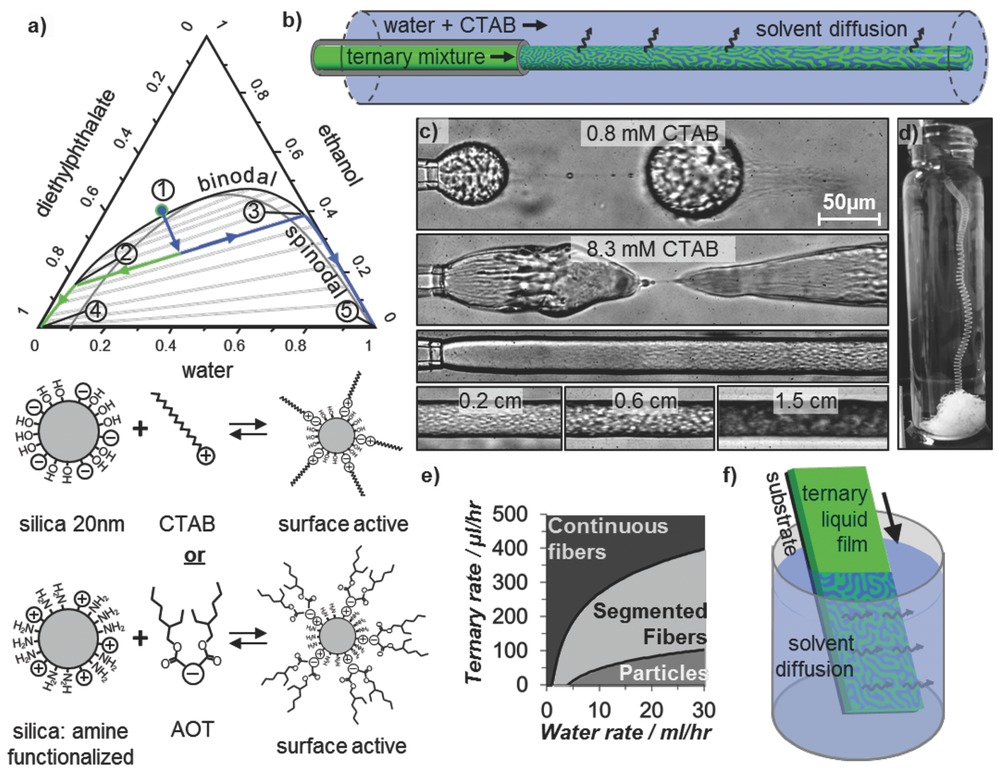
\includegraphics[scale = 5]{figures/introduction/STrIPS.jpg}
    \caption{Extrusion of the bijel casting mixture into a non-solvent bath, followed by removal of solvent from 
             the casting mixture through diffusion, demonstrating the working principal of STrIPS. \cite{haase_continuous_2015}. 
             Reprint of Figure 2 from 
             \textit{Haase, M. F.; Stebe, K. J.; Lee, D. Continuous Fabrication of Hierarchical and Asymmetric Bijel Microparticles, Fibers, and Membranes by Solvent Transfer-Induced Phase Separation (STRIPS). Advanced Materials 2015, 27 (44), 7065-7071}
             with permission from Wiley-VCH Verlag GmbH \& Co. KGaA under license number 5913140219015}
    \label{fig:strips}
\end{figure}

% Vapor-induced phase separation (VIPS) offers another solvent-removal-based technique for bijel synthesis \cite{wang_scalable_2020}. In this approach, a quaternary mixture containing particles, a solvent, 
% and two partially miscible liquids is prepared. Careful selection of component identities and ratios ensures that evaporation of the solvent drives the system through its critical point, inducing spinodal 
% decomposition. A representative system uses water and hexanediol diacrylate, solvated by ethanol. As ethanol evaporates at room temperature, phase separation and bijel formation occur. VIPS is compatible 
% with spray or blade coating techniques but is limited by the temperature dependence of surface tension, restricting solvent options to those that vaporize readily at ambient conditions.

% In contrast to methods relying on spinodal decomposition, homogenization uses shear to coalesce domains of immiscible fluids, resulting in a bicontinuous structure that mimics a bijel 
% \cite{huang_bicontinuous_2017, cai_bijels_2017}. This approach is particularly effective for nanoparticles under 50 nm and supports various particle shapes. Shear promotes limited coalescence 
% of droplets; as coarsening proceeds, particles adsorb at the interface. Once the interfacial area is saturated with particles, jamming occurs, locking the microstructure in place. Tuning can be 
% achieved by modifying particle contact angles (e.g., via surfactants) or adjusting the viscosity of the fluid phases using additives like oligomers.
% Despite these advances, a persistent limitation is that bijel microstructure remains tightly coupled to the composition of the casting mixture and the kinetics of phase separation. Achieving controlled 
% morphology often requires fine-tuning of fluid concentrations or external conditions, which may not be feasible for all applications \cite{haase_continuous_2015, reeves_particle-size_2015}.

Despite these advances, a limitation is that bijel microstructure remains tightly coupled to the composition of the casting mixture and the kinetics of phase separation. Achieving controlled 
morphology often requires fine-tuning of fluid concentrations or external conditions, which may not be feasible for all applications \cite{haase_continuous_2015, reeves_particle-size_2015}.
The ability to tune these structural features would significantly expand the versatility and functionality of bijel-based systems.
In many of the proposed applications such as water filtration membranes or drug delivery 
platforms, the morphology of the material plays a critical role in determining key functional properties, including back pressure, species selectivity, and transport dynamics
\cite{vanoli_bijels_2022, thorson_bijel-templated_2019, khan_nanostructured_2022}.

Stimuli-responsive strategies present a promising avenue for achieving post-synthetic or in situ control over bijel microstructures. External triggers such as magnetic fields, pH, and temperature have 
been extensively studied in the context of Pickering emulsions to modulate droplet behavior and morphology \cite{tham_magnetophoresis_2021, cui_stabilizing_2013}. In these systems, magnetically 
responsive particles have been used to manipulate, deform, and control the coalescence of droplets, as illustrated in Figure~\ref{fig:magnetophoresis_droplet}. Magnetic 
fields offer a targeted method for manipulating the behavior of particles making them of particular interest. 
However the application of such dynamic control strategies to bijels remains relatively underexplored. Prior studies involving magnetic fields applied to bijels stabilized with spherical particles 
have shown limited success in modifying the microstructure, due to the isotropic nature of the stabilizing particles \cite{kim_bijels_2010}. 
% In comparison, electric fields have demonstrated a 
% greater capacity to influence bijel morphology, suggesting that the type of stimulus and particle properties play critical roles in enabling responsive behavior \cite{carmack_tuning_2018}. 

\begin{figure}
    \centering
    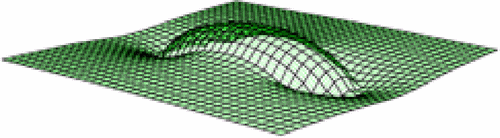
\includegraphics[scale = 0.5]{figures/literature_review/interfacial_curvature.png}
    \caption{Quadropolar capillary interactions around prolate ellipsoidal particles caused by interfacial deformations 
             around the particle. Reprinted Figure 4 with permission from
             \textit{Loudet, J. C.; Alsayed, A. M.; Zhang, J.; Yodh, A. G. Capillary Interactions Between Anisotropic Colloidal Particles. Phys. Rev. Lett. 2005, 94 (1), 018301}
             Copyright 2025 by the American Physical Society.}
    \label{fig:anisotropic_particle_interface}
\end{figure}

Anisotropic particles exhibit shape-dependent interfacial behavior due to their ability to deform fluid interfaces while maintaining zero mean curvature, as seen in 
(Figure~\ref{fig:anisotropic_particle_interface}) \cite{loudet_capillary_2005, cheng_shape-anisotropic_2013}. These deformations generate multipolar capillary interactions, which can be harnessed 
for curvature-guided migration and directed assembly at fluid interfaces \cite{cavallaro_curvature-driven_2011, read_dimerization_2020, sharifi-mood_curvature_2015}. Simulations have shown that 
ellipsoidal particles can adopt multiple metastable orientations depending on external perturbations and interfacial constraints \cite{gunther_lattice_2013}. When used as stabilizers in bijels, 
ellipsoidal particles produce finer domains than spherical particles at equivalent volume fractions, a result of their higher surface area-to-volume ratio and more efficient interfacial coverage 
\cite{gunther_timescales_2014}.

The dynamics of ellipsoid-stabilized bijels display additional dynamics and droplet bridging, not observed in their spherical counterparts \cite{gunther_timescales_2014, witt_bijel_2013}. Initially, 
particles adsorb and align with the interface, followed by a slower reorganization phase driven by capillary interactions between particles \cite{gunther_timescales_2014}. Experimental results 
confirm that the domain size in rod and ellipsoid stabilized bijels still follows the scaling law $L \propto \frac{1}{\phi_p}$, though the proportionality constant depends on particle geometry 
\cite{hijnen_bijels_2015, madivala_exploiting_2009, daware_emulsions_2015}.

The geometry of the stabilizing particles plays a key role in determining rheological behavior. Madivala et al. showed that Pickering emulsions stabilized with rod-like particles had enhanced 
stability under shear, with greater resistance observed as particle aspect ratio increased \cite{madivala_exploiting_2009}. This enhancement was attributed to improved interfacial coverage 
and capillary interactions induced by interface deformations, which reinforced the particle monolayer. Similarly, emulsions stabilized by graphene nanosheets exhibited higher viscosity and 
viscoelasticity compared to those stabilized by spherical particles, underscoring the importance of particle shape \cite{imperiali_simple_2014}. The elasticity of the interface has also been 
shown to depend on the nature of the particle stabilizer used \cite{sun_assembly_2013}.

The rheological properties of bijels are of fundamental importance due to their direct influence on both fabrication and application. For instance, STrIPS fabrication relies on the controlled 
flow of a casting mixture into a solvent bath, necessitating precise knowledge of the material's rheology to optimize processing parameters \cite{haase_situ_2016, haase_continuous_2015}. 
In applied systems such as cross-flow reactors, the mechanical stability of the particle monolayer is critical; failure under shear or compositional gradients can limit performance 
\cite{boakye-ansah_controlling_2020}. Under constant shear, bijels exhibit shear-thinning behavior, which at moderate shear rates is well described by the Herschel-Bulkley model 
\cite{macmillan_rheological_2019, wang_morphology_2023}. At higher shear rates, the internal structure of the bijel is disrupted, leading to a transition toward Newtonian 
flow behavior \cite{cai_bijels_2017, bonaccorso_shear_2020}.

\begin{figure}
    \centering
    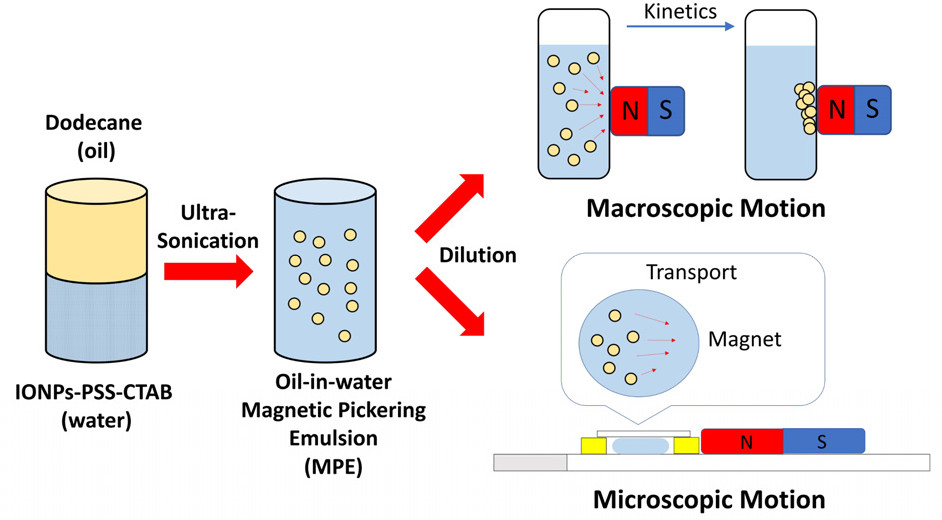
\includegraphics[scale = 1.5]{figures/introduction/magnetophoresis_emulsion.jpeg}
    \caption{Enhanced oil recovery of oil from water using magnetically responsive emulsion stabilizers, allowing for 
             locomotion and controlled coalescence of cargo from a matrix phase using magnetic fields. Reprint of the graphical abstract from
             \textit{Tham, F. K.; Ng, W. M.; Leong, S. S.; Yeap, S. P.; Low, S. C.; Lee, H. L.; Lim, J. Magnetophoresis of Magnetic Pickering Emulsions Under Low Field Gradient: Macroscopic and Microscopic Motion. Langmuir 2021, 37 (5), 1811-1822}
             Reprinted (adapted) with permission from Langmuir 2021, 37, 5, 1811-1822. Copyright 2025 American Chemical Society.}
    \label{fig:magnetophoresis_droplet}
\end{figure}

Introducing magnetic responsiveness into anisotropic particles offers a strategy for controlling their behavior at fluid interfaces. Such particles can be fabricated via surface deposition of 
magnetic materials or synthesized as core-shell structures with magnetic cores and non-magnetic shells \cite{fei_magneto-capillary_2020, nakayama_stimuli-responsive_2018}. The interplay between 
magnetic and capillary interactions governs particle orientation in response to external magnetic fields. According to Bresme-Faraudo theory, a neutrally wetting ellipsoidal particle at an 
interface experiences competing forces: the magnetic field seeks to reorient the particle's magnetic dipole moment, while capillary forces resist deformation away from the interface plane 
\cite{bresme_orientational_2007, davies_interface_2014}.

\begin{figure}
    \centering
    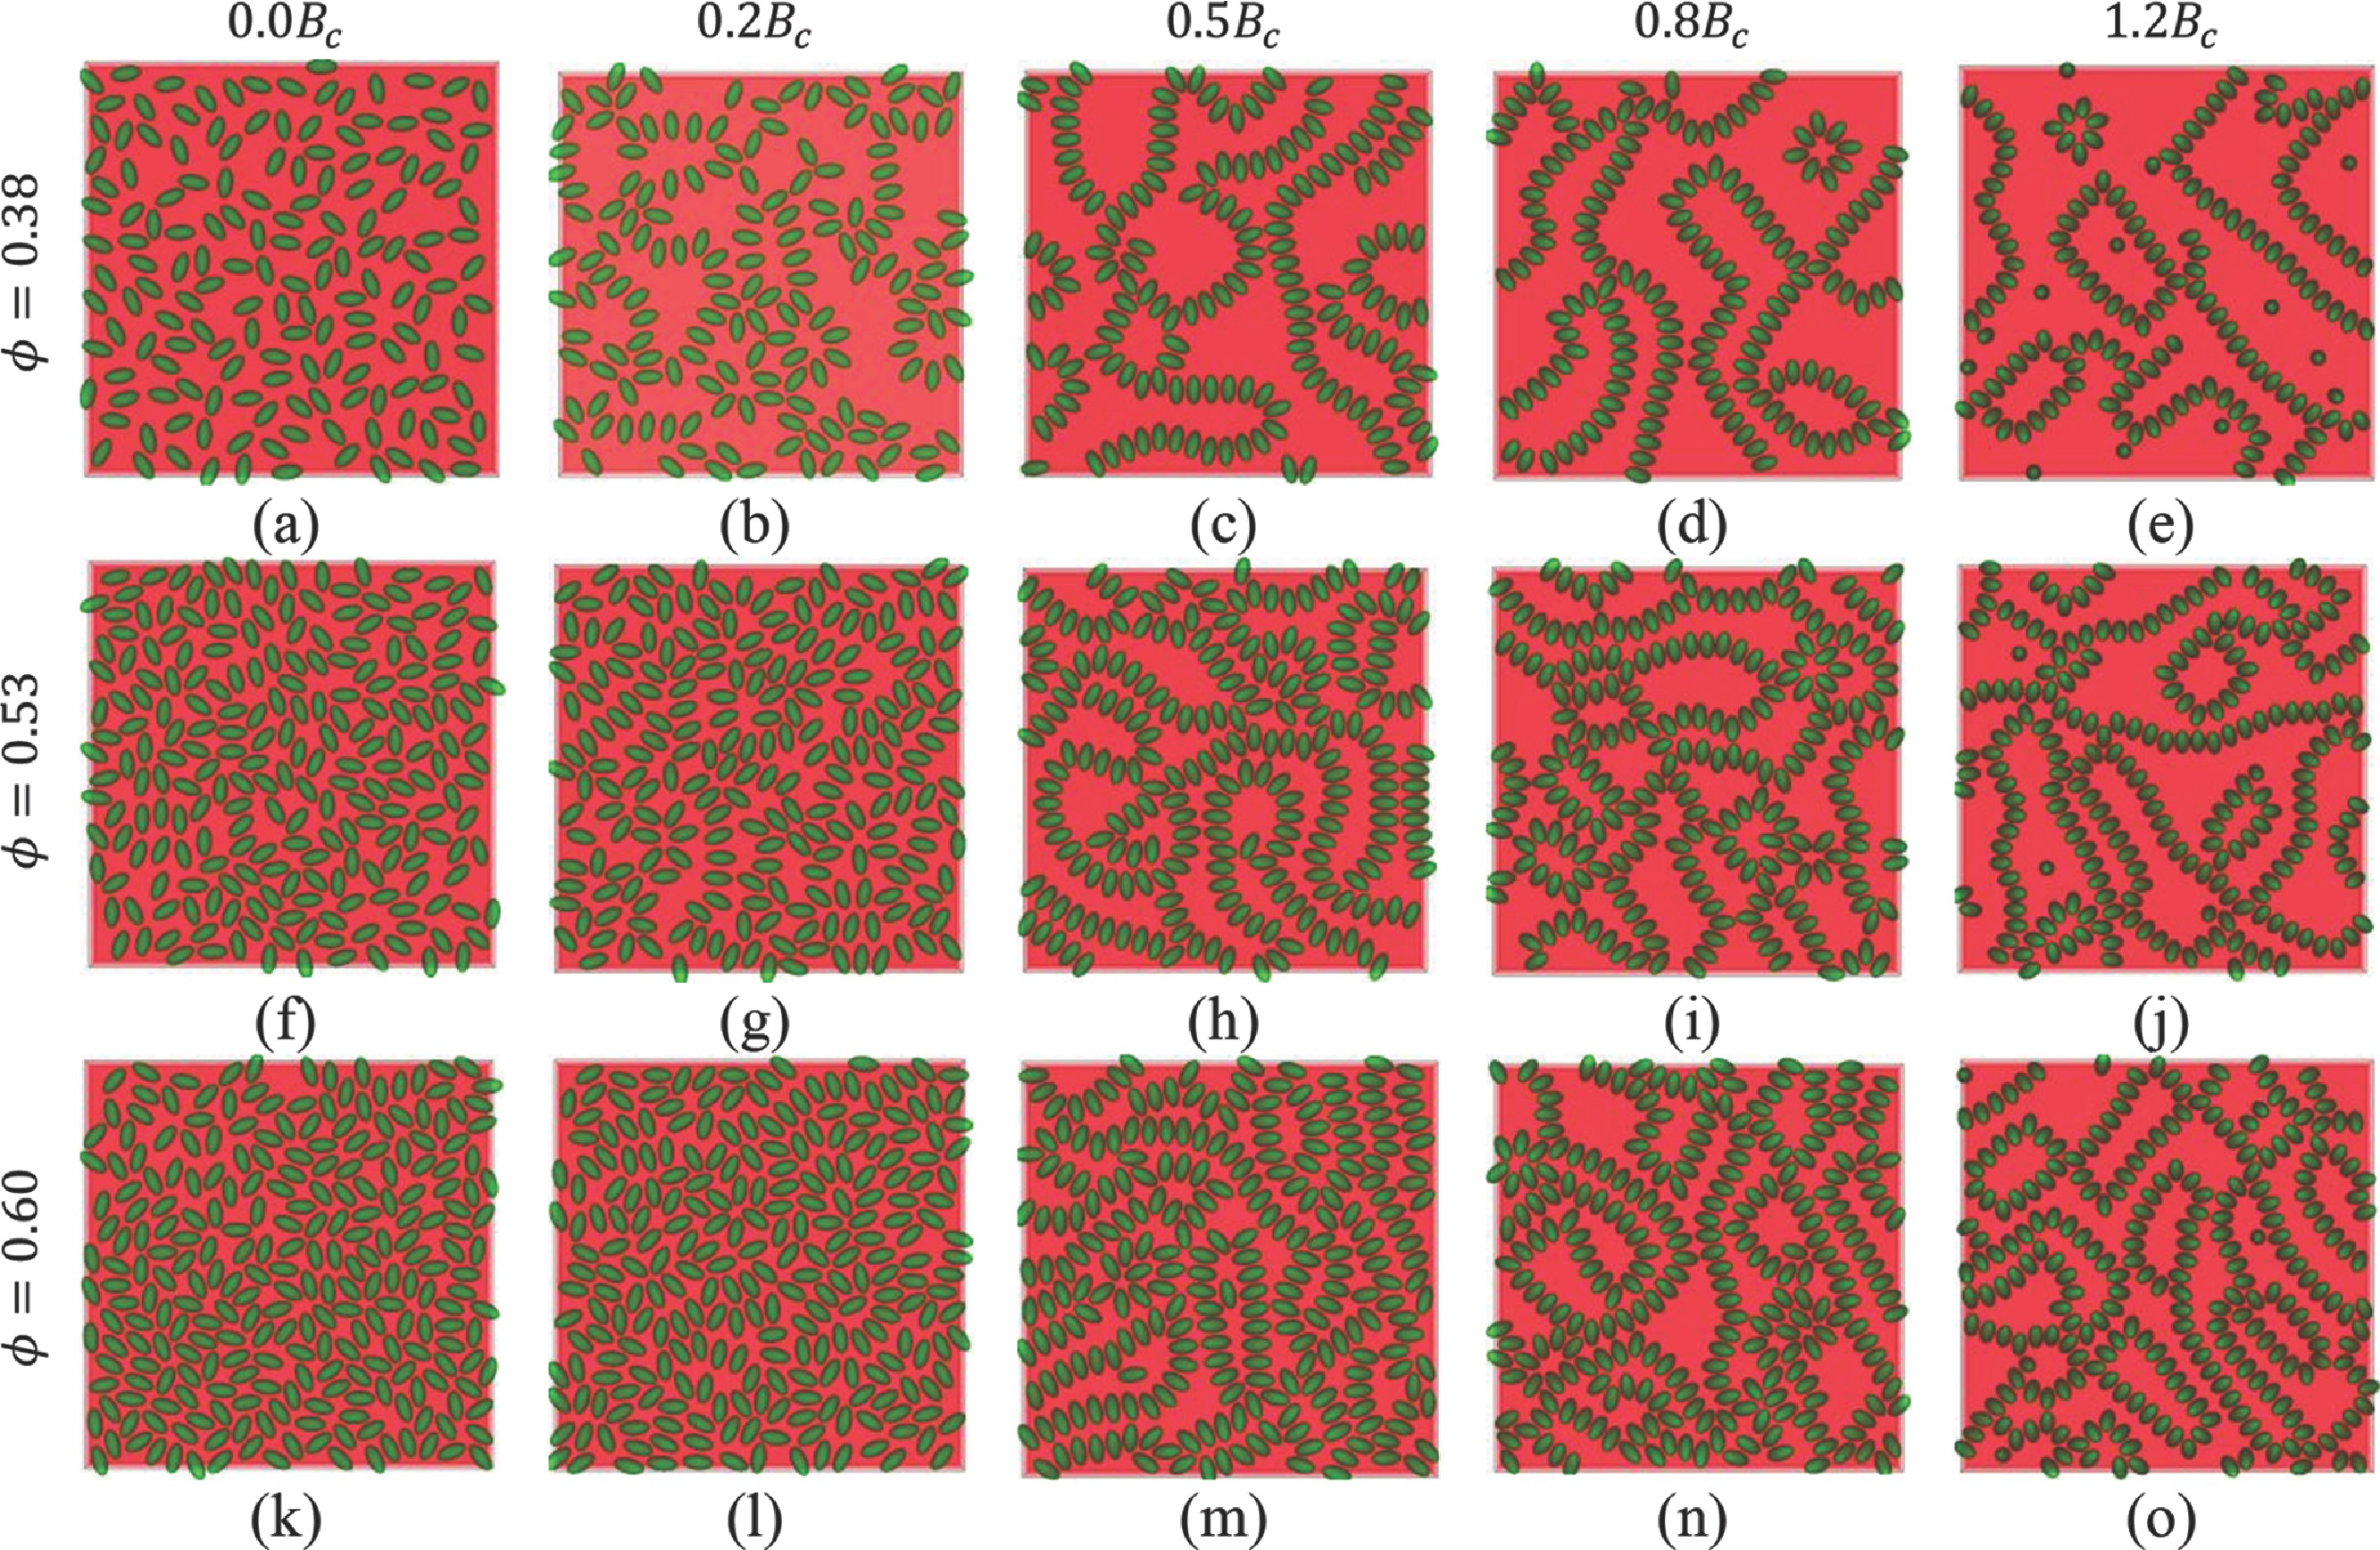
\includegraphics[scale = 0.4]{figures/introduction/anisotropic_particles_assembly.jpg}
    \caption{Assembly of prolate particles on a flat interface at various interfacial coverages and field strengths,
             showing the self assembly into chains that ellipsoidal particles can undergo under applied magnetic fields at
             interfaces. Reprint of Figure 3 from
             \textit{Davies, G. B.; Krüger, T.; Coveney, P. V.; Harting, J.; Bresme, F. Assembling Ellipsoidal Particles at Fluid Interfaces Using Switchable Dipolar Capillary Interactions. Advanced Materials 2014, 26 (39), 6715-6719}
             with permission from Wiley-VCH Verlag GmbH \& Co. KGaA under the Creative Commons CC BY license.}
    \label{fig:anisotropic_assembly}
\end{figure}

The equilibrium and metastable orientations adopted by anisotropic particles are functions of particle aspect ratio, surface wettability, and interfacial tension 
\cite{morgan_understanding_2013, newton_influence_2014}. Studies on cuboidal hematite particles at oil-water interfaces demonstrate multiple stable and metastable states, where particles align 
their major or minor axes relative to the interface depending on their geometry and energy landscape. Lattice Boltzmann simulations support these observations, showing how particle shape influences 
and contact angle affect the energy required to detach a particle from an interface \cite{davies_detachment_2014}. 
Magnetic fields can perturb these equilibria by exerting torque on the particles, reorienting them along the field direction. 
Experiments confirm that magnetic ellipsoids can be reconfigured at the interface, enabling controlled switching between metastable and stable configurations.
As more particles interact under a magnetic field, their mutual dipolar interactions lead to the formation of linear chains or clusters on flat interfaces 
\cite{davies_assembling_2014, newton_capillary_2018}. The final arrangement is influenced by particle concentration, field strength, and local capillary geometry. 

These effects enable magnetic field driven droplet deformation, coalescence and 
motility of Pickering Emulsions, demonstrating the potential for real-time, field-controlled manipulation of interfacial structures \cite{melle_pickering_2005, tham_magnetophoresis_2021}.
The applied field can also alter the materials rheological response as the stabilizing particles reorient and reorganize at the interface
enabling reversible transitions between fluid-like and gel-like states. \cite{qiao_magnetorheological_2012, melle_pickering_2005}. 
Such behavior is particularly advantageous for applications in enhanced oil recovery, drug delivery, and soft robotics, where adaptable and 
reconfigurable materials are essential \cite{tham_magnetophoresis_2021}.


This dissertation investigates the potential of magnetically responsive ellipsoidal particles to enable stimuli-responsive control over bijel microstructure. Specifically, it examines whether magnetic 
fields applied during or after bijel formation can induce meaningful structural changes, and how these changes, in turn, influence the rheological behavior of the resulting material. Upon application of
a constant magnetic field, a torque will be imparted which will rotate the particles at the interface towards the direction of the magnetic field. This reorientation is hypothesized to impart
structural changes in the bijel. Carmack and Millet identified that the formation of particle chains was shown to play a critical role in phase separation dynamics. These chains acted as 
nucleation sites, guiding the development of fluid domains and influencing average channel diameter and particle localization at interfaces. These findings suggest that external fields, 
particularly when coupled with anisotropic particles, offer a promising route toward responsive and reconfigurable bijel architectures.

The remainder of this dissertation is organized as follows. Chapter 2 reviews important background relevant to bijel formation and simulations of bijels.
Chapter 3 details the physical model and the simulation methods used to solve these physics, including the Lattice Boltzmann Method implementation. Chapter 4 investigates the effects 
of magnetic fields applied during bijel formation, analyzing their influence on domain structure and particle orientation. Chapter 5 performs quantitative microstructural characterization of the effects
of magnetic fields on the microstructure of bijels. Chapter 6 explores post-formation responsiveness, examining whether the microstructure of a stimuli responsive bijel can be modified
post-synthesis. Chapter 7 assesses the rheological implications of these structural changes, with particular attention to yield stress and shear-thinning behavior. Finally, Chapter 8 summarizes 
key findings, discusses their implications for the design of tunable porous materials, and outlines potential directions for future research.